\documentclass[main]{subfiles}
\begin{document}

%@@@@@@@@@@@@@@@@@@@@@@@@@@@@@@
% Main Topics: Introduction 20.09.2018
% Lecturer: Matthew Cook
% author: Vanessa Leite - base document from benelot/eth-intro-to-neuroinformatics-summary

\section{Neuroinformatics}

\subsection{Introduction}
\begin{itemize}[noitemsep,nolistsep]
	\item Human brain on average: $1.5 kg$ weight, $1.2 l$ volume.
	\item Human brains are large, but by far not the largest (for instance, elephants and whales have bigger brains).
	\item The brain mainly is there to receive stimuli from the environment, encode it, do sensory integration and finally decode to make movements, actions and decisions.
	\item The cells (neurons) that make up brains are very similar between species.
	\item Some neuron types occur in specific parts of the brain and it is consistent between species.
	\item A neuron is a processing unit that receives electrical input and generates electrical output.

\end{itemize}
\begin{figure}[htbp]
	\centering
	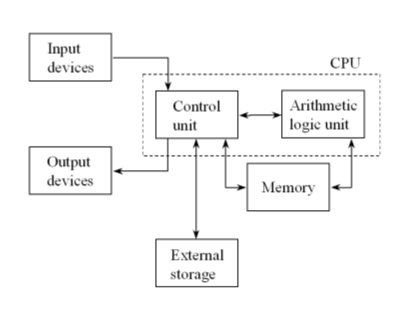
\includegraphics[scale=0.6]{1_2.jpg}
 	\caption{Turing Machine / CPU}
\end{figure} 

\paragraph{How information is processed in the brain?}
We can consider many levels when we talk about the brain processing information. From the highest to the lowest level: behavior $\rightarrow$ system and pathways $\rightarrow$ circuits $\rightarrow$ neurons $\rightarrow$ microcircuits $\rightarrow$ synapses $\rightarrow$ membrane potential (molecules and ions). \\

\textbf{Differences between a brain and a computer (what the brains have):}
\begin{itemize}[noitemsep,nolistsep]
	\item Massive parallelism
	\item Constantly adapting
	\item Chemical signaling
	\item Unreliable units (brain is noisy compared to a computer)
	\item Analog computation
	\item Robust to damage
	\item Very energy efficient
	\item Memory fixed in place (as part of each processing unit).
\end{itemize}
\textbf{Similarities between a brain and a computer:}
\begin{itemize}[noitemsep,nolistsep]
	\item Process information
	\item Logical operations
	\item Memory
	\item Use electrical (digital) signaling
	\item Can learn from inputs
	\item Consume energy
\end{itemize}

\paragraph{Easy vs Dificult tasks}
Things that we can do and computer can't, change over time. Things that are easy to humans can be hard to a computer, mostly because we don't know how to simulate a brain. We do things without think consciously about it.

\begin{itemize}
\item It is comparatively easy to make computers exhibit adult level performance on intelligence tests or playing checkers, and difficult or impossible to give them the skills of a one-year-old when it comes to perception and mobility.” – Hans Moravec
\end{itemize}

\paragraph{Neurons structure}
\begin{itemize}[noitemsep,nolistsep]
	\item Membrane: Separates inside from outside.
	\item Soma: Cell body, contains nucleus and organelles.
	\item Dendrites: Connect to soma, provide inputs to soma.
	\item Axons: Connects to soma, conducts away from soma. Often myelinated and ends in synapses. Carries output.
	\item Synapse: Pre- and postsynaptic terminals, transmit information between neurons.
	\item In the order of magnitude, there are about 10'000 synapses per neuron.
\end{itemize}

\textbf{Other facts}
\begin{itemize}[noitemsep,nolistsep]
	\item An 83000-Processor supercomputer can only match $1\%$ of the human brain.
	\item C. Elegans (worm) has 302 nerve cells, a frog 16M, a cat 1B and a human 85B.
	\item Human brain project aims to simulate the entire human brain on computers.
	\item More efficient simulations of brain behavior by Neurogrid or IBM TrueNorth.
	\item Number of neurons in human brain: $\sim10^{11}$, synapses: $\sim10^{15}$.
	\item Number of genes in human genome: $\sim$25000.
	\item WindowsXP contains more code (1.5Gb) for operating a personal computer than DNA ($\sim$750Mb) to generate life.
	\item Deep Neural Networks were inspired by the brain in the beggining but it is not like the brain (neurons) works.
	
\end{itemize}

\end{document}
